%%%%%%%%%%%%%%%%%%%%%%%%%%%%%%%%%%%%%%%%%%%%%%%%%%%%%%%%
%%%%%%%%%------RMIT SPACE POSTER------------%%%%%%%%%%%%
%%%%%%%%%%%%%%%%%%%%%%%%%%%%%%%%%%%%%%%%%%%%%%%%%%%%%%%%
%%%%%%%%%%%%%%%%%%%%%%%%%%%%%%%%%%%%%%%%%%%%%%%%%%%%%%%%
% a0poster Portrait Poster
%
% The a0poster class was created by:
% Gerlinde Kettl and Matthias Weiser (tex@kettl.de)
% 
% License:
% CC BY-NC-SA 3.0 (http://creativecommons.org/licenses/by-nc-sa/3.0/)
%
% Author/Designer: Timothy Kodikara
%
%% Note: CRC and SERC logos are included in the /figures folder if you might want to use them.
%%%%%%%%%%%%%%%%%%%%%%%%%%%%%%%%%%%%%%%%%
%----------------------------------------------------------------------------------------
%	PACKAGES AND OTHER DOCUMENT CONFIGURATIONS
%----------------------------------------------------------------------------------------
\documentclass[a0,portrait]{a0poster}
%%
\usepackage[top=5cm, bottom=0.3cm, left=5cm, right=3cm]{geometry}
\usepackage[compact]{titlesec}
\usepackage{multicol} % This is so we can have multiple columns of text side-by-side
\columnsep=100pt % This is the amount of white space between the columns in the poster
\columnseprule=10pt % This is the thickness of the blue line between the columns in the poster
\usepackage[svgnames]{xcolor} % Specify colors by their 'svgnames', for a full list of all colors available see here: http://www.latextemplates.com/svgnames-colors
%\usepackage{times} % Use the times font
\usepackage{palatino} % Uncomment to use the Palatino font
\usepackage{xkeyval}
\usepackage{graphicx} % Required for including images
\setlength{\abovecaptionskip}{5pt plus 5pt minus 3pt}
\graphicspath{{figures/}} % Location of the graphics files
\usepackage{booktabs} % Top and bottom rules for table
\usepackage[font=small,labelfont=bf]{caption} % Required for specifying captions to tables and figures
\usepackage{amsfonts, amsmath, amsthm, amssymb} % For math fonts, symbols and environments
\usepackage{csquotes}
\usepackage{wrapfig} % Allows wrapping text around tables and figures
%\usepackage[pdftex]{color}
\def\columnseprulecolor{\color{Orange}}%
\usepackage{framed}
\colorlet{frameborder}{Orange}
%----------------------------------------------------------------------------------------
%	POSTER HEADER 
%----------------------------------------------------------------------------------------
% The header is divided into three boxes:
% The widths of these boxes can be easily edited to accommodate your content as you see fit
\begin{document}
%\hspace*{0.2cm}
\begin{minipage}[c]{\linewidth}
\vspace{0.1cm}
\noindent\makebox[\textwidth][c]{
\begin{minipage}[c]{0.10\linewidth}
\vspace{0pt}\raggedright
\hspace{1cm}

\includegraphics[width=1.5\linewidth]{SUSTech}
\end{minipage}
\hfill
\begin{minipage}[c]{0.70\textwidth}
\centering
\Huge \color{NavyBlue} \textbf{Automated EEG-based major depress disorder detection through transformer-based network}\\[0.5cm]
\large \color{Black} \textbf{Ziyan Zhang$^{1}$, Zhe Cao$^{1}$, Weiqi Ruan$^{1}$}\\[0.2cm] % Author(s)
\small 1. Institute for Quantum Science and Engineering, SUSTech, Shenzhen, China\\[0.1cm] % University
\small \texttt{Correspondence: 12132873@mail.sustech.edu.cn}\\
\small \texttt{12132834@mail.sustech.edu.cn}\\
\small \texttt{1023104572@qq.com}\\
\end{minipage}
%\hfill
\begin{minipage}[c]{0.15\textwidth}
\vspace{0pt}\raggedleft

\includegraphics[scale=1,width=1.1\linewidth]{BME5012}
\hspace{1cm}
\end{minipage}}
\\[0.1cm]%
% A bit of extra whitespace between the header and poster content
%----------------------------------------------------------------------------------------
\color{Orange}\setlength\FrameRule{10pt}
\begin{framed}
\vspace{0.5cm}
\begin{multicols}{2} % This is how many columns your poster will be broken into, a portrait poster is generally split into 2 columns
%----------------------------------------------------------------------------------------
%	INTRODUCTION
%----------------------------------------------------------------------------------------
\color{Black}
\section*{Introduction}
In recent years, deep learning has been extensively used for arbitrary diagnosis of many mental diseases based on EEG or fMRI, including epilepsy$^1$, seizure prediction$^2$, Alzheimer's disease$^3$, etc. Simultaneously, depression is a common illness worldwide, with an estimated 3.8\% of the population affected, including 5.0\% among adults and 5.7\% among adults older than 60 years. Over 700,000 people die due to suicide caused by the depression every year. $^4$  However, it can be effectively diagnosed and treated in early period. A schematic comparison of synapses from a healthy subject and a depressed subject is presented in Fig. 1.\\
%\begin{wrapfigure}{R}{0.25\textwidth}
\begin{center}
\hspace*{\fill}
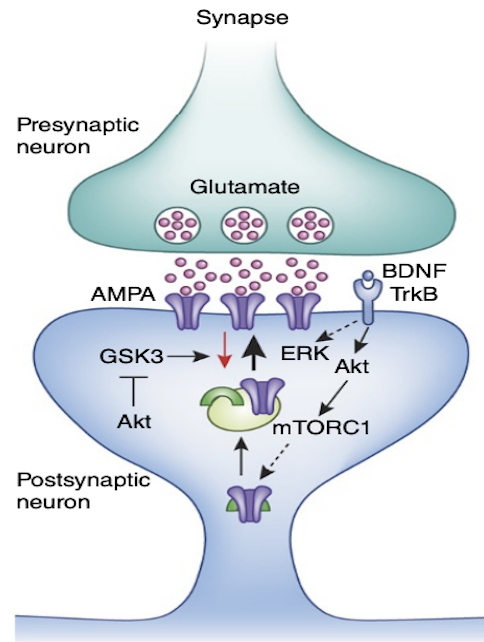
\includegraphics[width=0.4\linewidth]{figures/normal_syn}
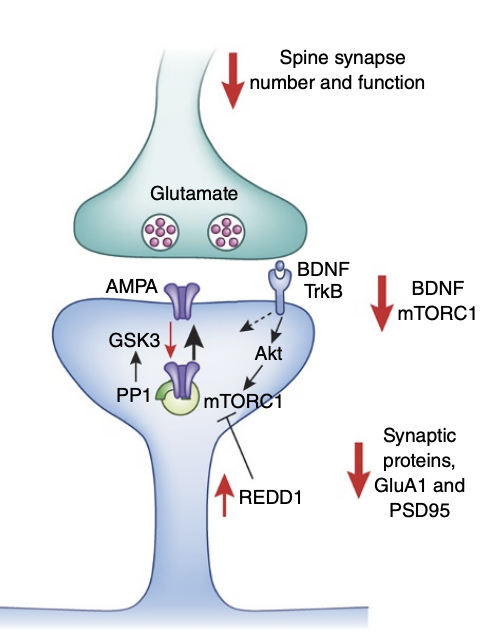
\includegraphics[trim={0 0.9cm 0 0},clip,width=0.49\linewidth]{figures/abnormal}
\captionof{figure}{\color{Green}A schematic comparison of synapses of a healthy subject (left) and a depressed patient (right)$^5$.}
\label{IGSMap}
\end{center}
In this work, we presented an EEG-based major depress disorder detection neural network based on GPT-3. It takes EEG signal as input and outputs its predication graded with None, Mild, Moderate and Severe based on the severity of symptoms. We trained this network with 128 channels resting signal obtained 24 major depressive disorder subjects and 29 healthy control subjects, ranging from 16 - 52 years old$^6$. This model was tested by various public datasets, the accuracy and f1 score can reach about 0.9. Additionally, we compared our network with naive CNN and RNN, we can induct that our model performs better.
%----------------------------------------------------------------------------------------
%	METHODS
%---------------------------------------------------------------------------------------- 
\color{Black}
\section*{Data and Methods}
%\begin{wrapfigure}{R}{0.25\textwidth}
%\centering
%\end{wrapfigure}
The data being used in this work is an open-source EEG dataset from UAIS Lab, Lanzhou University, China$^6$. The dataset contains traditional 128-electrodes EEG signals as well as audio data from clinically depressed patients and matching normal controls. The EEG signals of 53 subjects were recorded in resting state \& under stimulation.  \\
\begin{center}

\includegraphics{figures/placeholder}
\captionof{figure}{\color{Green}Loreteur sint occaecat cupidatat non proident, sunt in culpa qui officia deserunt mollit anim id est laborum.}
\label{STECchart}
\end{center}
%\hspace{0.1cm}$\circ$ Sdfshd d: 25\textendash31 January, 2015;\\
%\hspace{0.1cm}$\circ$ Redfshdghgons (Fig.\ref{IGSMap}): Lorem ipsum dolor sit amet, consectetur adipiscing elit, sed;\\
%\hspace{0.1cm}$\circ$ Geomagnetic activity: Kp $<$ 4 throughout the study period;\\
%\hspace{0.1cm}$\circ$ Analysis: Two types of accuracy and;\\
%\hspace{0.1cm}$\circ$ GIR: Lorem ipsum dolor sit amet, consectetur adipiscing elit, sed do eiusmod tempor;\\
%\hspace{0.1cm}$\circ$ AGD: Lsunt in culpa qui officia deserunt mollit anim id est laborum.\\
The pre-processing of the raw EEG signal contains 3 parts, 
\begin{enumerate}
\item Segmenting
\item Band-pass filtering
\item Standarlization
\end{enumerate}
The data is segmented into trials as $C_{eeg}*T$, where $C_{eeg}$ is the number of EEG channels and $T$ is the sample points. Then we add band-pass filter data to $[4,40]Hz$ to remove high and low-frequency noise. After that we apply standard normalization to relive the fluctuation and non-stationarity  as $$X={x-\mu}/{\sqrt{\sigma}^2}$$Additionally, we give a feasible way based on CSP usage to improve the difference of the original signal and maintain the temporal information.\\
\begin {center}
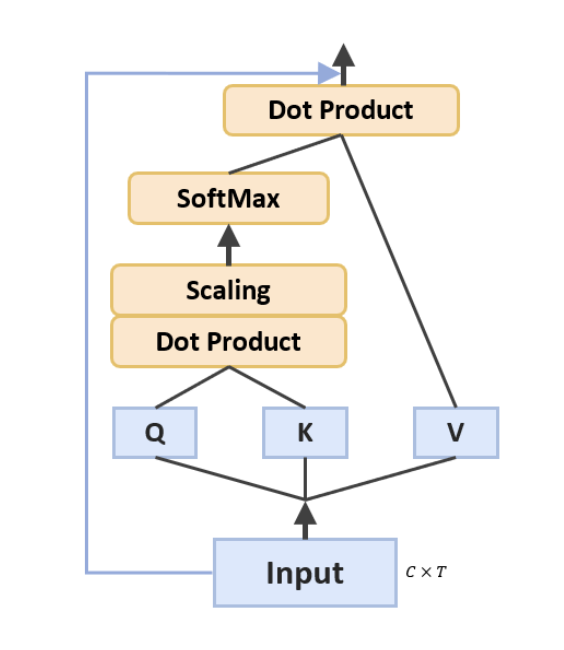
\includegraphics{figures/dot}
\captionof{figure}{\color{Green}The calculation process of spatial feature-channel attention}
\label{dot}
\end{center}
We proposed a method of feature channel weighting inspired by the scaled dot-product. As illustrated in Fig.\ref{dot}. \\
\hspace{0.1cm}$\circ$ Lorem ipsum dolor sit amet, consectetur adipiscing elit, sed do eiusmod tempor.\\
Lorem ipsum dolor sit amet, consectetur adipiscing elit, sed  3\,mm/$\sqrt[]{hour}$. The.
%----------------------------------------------------------------------------------------
%	RESULTS
%---------------------------------------------------------------------------------------- 
\color{Black}
\section*{Results}
Fig.-\ref{BIvar} compares tLorem ipsum dolor sit amet, consectetur adipiscing elit, sed do eiusmod tempor incididunt ut labore et dolore magna aliqua. Ut enim ad minim veniam, quis nostrud exercitation ullamco laboris nisi ut aliquip ex ea commodo consequat. Duis aute irure dolor in reprehenderit in voluptate velit esse cillum dolore eu fugiat nulla pariatur. Excepteur sint occaecat cupidatat non proident, sunt in culpa qui officia deserunt mollit anim id est laborum.
\begin{center}

\includegraphics[width=0.8\linewidth]{figures/placeholder}
\captionof{figure}{\color{Green}Cdfhfghgf R (gfhfgh) and GDDDE.}
\label{BIvar}
\end{center}
Lorem ipsum dolor sit amet, consectetur adipiscing elit, sed do eiusmod tempor incididunt ut labore et dolore magna aliqua pariatur. Excepteur sint occaecat cupidatat non proident, sunt in culpa qui officia deserunt mollit anim id est laborum 705 valid (CT$\neq$0) improvements in CT.
\begin{center}

\includegraphics[width=0.9\linewidth]{figures/placeholder}
\captionof{figure}{\color{Green} Duis aute irure dolor in reprehenderit in voluptate velit esse cillum dolore eu fugiat nulla pariatur. Excepteur sint occaecat cupidatat non proident, sunt in culpa qui officia deserunt mollit anim id est laborum.}
\label{ALICerros}
\end{center}
Fig.-\ref{ALICerros} illustrates Lorem ipsum dolor sit amet, consectetur adipiscing elit, sed do eiusmod tempor incididunt ut labore et dolore magna aliqua. Ut enim ad minim veniam, quis nostrud exercitation ullamco laboris nisi ut aliquip ex ea commodo consequat. Duis aute irure dolor in reprehenderit in voluptate velit esse cillum dolore eu fugiat nulla pariatur. Excepteur sint occaecat cupidatat non proident, sunt in culpa qui officia deserunt mollit anim id est laborum.\\
Lorem ipsum dolor sit amet, consectetur adipiscing elit, sed do eiusmod tempor incididunt ut labore et dolore magna aliqua. Ut enim ad minim veniam, quis nostrud exercitation ullamco laboris nisi ut aliquip ex ea commodo consequat. Duis aute irure dolor in reprehenderit in voluptate velit esse cillum dolore eu fugiat nulla pariatur. Excepteur sint occaecat cupidatat non proident, sunt in culpa qui officia deserunt mollit anim id est laborum
\begin{center}

\includegraphics[width=0.9\linewidth]{figures/placeholder}
\captionof{figure}{\color{Green}VLorem ipsum dolor sit amet, ulpa qui officia deserunt mollit anim id est laborumime.}
\label{GIMupdown}
\end{center}
\vspace{0.1cm}
\begin{center}

\includegraphics[width=0.9\linewidth]{figures/placeholder}
\captionof{figure}{\color{Green}Lorem ipsum dolor sit amet, consectetur adipiscing elit, sed do eiusmod tempor.}
\label{GIMlatlon}
\end{center}
%----------------------------------------------------------------------------------------
%	CONCLUSIONS
%----------------------------------------------------------------------------------------
\color{Black}
\section*{Summary}
Two typesLorem ipsum dolor sit amet, consectetur adipiscing elit, sed do eiusmod tempor incididunt ut labore et dolore magna aliqua. Uore eu fugiat nulla pariatur. Excepteur sint occaecat cupidatat non proident, sunt in culpa qui officia deserunt mollit anim id est laborum. In summary, we wish to highlight the following:\\ 
\hspace{0.1cm}$\circ$ text is derived from sections 1.10.33 of Cicero's De finibus bonorum et malorum;\\
\hspace{0.1cm}$\circ$ text is derived from sections 1.10.33 of Cicero's De finibus bonorum et malorum;\\
\hspace{0.1cm}$\circ$ text is derived from sections 1.10.33 of Cicero's De finibus bonorum et malorum;\\ 
\hspace{0.1cm}$\circ$ text is derived from sections 1.10.33 of Cicero's De finibus bonorum et malorum;\\
\hspace{0.1cm}$\circ$ text is derived from sections 1.10.33 of Cicero's De finibus bonorum et malorum;\\
\hspace{0.1cm}$\circ$ text is derived from sections 1.10.33 of Cicero's De finibus bonorum et malorum;\\
\hspace{0.1cm}$\circ$ text is derived from sections 1.10.33 of Cicero's De finibus bonorum et malorum.\\
text is derived from sections 1.10.33 of Cicero's De finibus bonorum et malorumtext is derived from sections 1.10.33 of Cicero's De finibus bonorum et malorumtext is derived from sections 1.10.33 of Cicero's De finibus bonorum et malorumtext is derived from sections 1.10.33 of Cicero's De finibus bonorum et malorumtext is derived from sections 1.10.33 of Cicero's De finibus bonorum et malorumtext is derived from sections 1.10.33 of Cicero's De finibus bonorum et malorumtext is derived from sections 1.10.33 of Cicero's De finibus bonorum et malorumtext is derived from sections 1.10.33 of Cicero's De finibus bonorum et malorum.
%----------------------------------------------------------------------------------------
%	ACKNOWLEDGEMENTS
%----------------------------------------------------------------------------------------
\section*{Acknowledgments}
\tiny \textnormal{This research was undertaken text is derived from sections 1.10.33 of Cicero's De finibus bonorum et malorumtext is derived from sections 1.10.33 of Cicero's De finibus bonorum et malorumtext is derived from sections 1.10.33 of Cicero's De finibus bonorum et malorum.}
\end{multicols}
%\textcolor{Orange}{\rule{\linewidth}{15pt}}
\vspace{0.5cm}
\end{framed}
\end{minipage}
%\hspace*{0.1cm}
\end{document}
%----------------------------------------------------------------------------------------
%%%%%%%%%%%%%%%%%%%%%%%%%%%%%%%%%%%%%%%%%%%%%%%%%%